\documentclass[tikz,border=4pt]{standalone}
\usepackage{amsmath}
\begin{document}
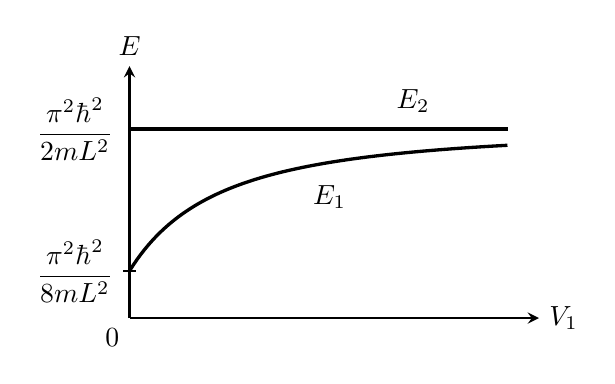
\begin{tikzpicture}[>=stealth, thick, scale=1.0]
  % Axes
  \draw[->] (0, 0) -- (5.2, 0) node[right] {$V_1$};
  \draw[->] (0, 0) -- (0, 3.2) node[above] {$E$};
  \node[below left] at (0, 0) {$0$};

  % E_2 = 4 E_1^{(0)} (constant)
  \draw[very thick] (0, 2.4) -- (4.8, 2.4);
  \node[left] at (-0.08, 2.4) {$\dfrac{\pi^2 \hbar^2}{2mL^2}$};
  \node[above] at (3.6, 2.48) {$E_2$};

  % E_1(V_1): starts at 0.6 (= 1/4 of 2.4), monotonically approaches 2.4
  \draw[very thick, domain=0:4.8, samples=100]
    plot (\x, {2.4 - 1.8 / (1 + 0.9*\x + 0.15*\x*\x)});
  \draw (-0.08, 0.6) -- (0.08, 0.6);
  \node[left] at (-0.08, 0.6) {$\dfrac{\pi^2 \hbar^2}{8mL^2}$};
  \node[below right] at (2.2, 1.82) {$E_1$};
\end{tikzpicture}
\end{document}
